\begin{frame}[t]{Cleaning Algorithms}
    \raisebox{10ex}{
    \begin{overlayarea}{0.36\textwidth}{3.5cm}
      \only<1>{
      \begin{itemize}
        \setlength\itemsep{1em}
        \item \code{white}{TailcutsImageCleaner}
        \item \code{white}{MARSImageCleaner}
        \item \code{white}{FACTImageCleaner}
        \item \code{white}{TimeConstrainedImageCleaner}
      \end{itemize}
      }
      \only<2>{
      \begin{itemize}
        \setlength\itemsep{1em}
        \item \code{white}{TailcutsImageCleaner}
        \item \code{white!50!black}{MARSImageCleaner}
        \item \code{white!50!black}{FACTImageCleaner}
        \item \code{white!50!black}{TimeConstrainedImageCleaner}
      \end{itemize}
      }
      \only<3>{
        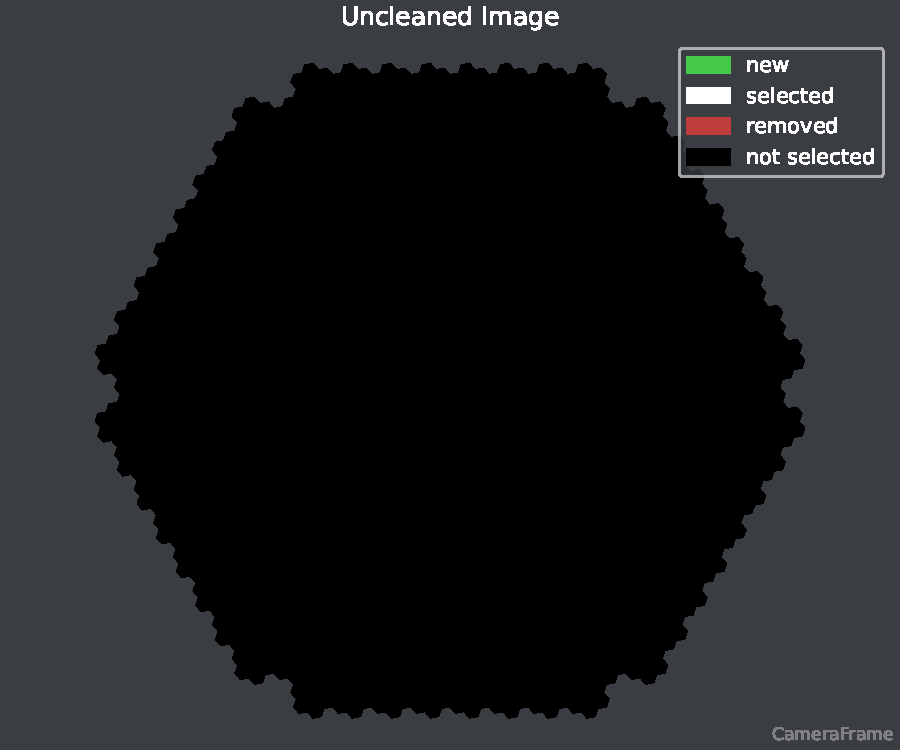
\includegraphics[width=\textwidth]{plots/cleaners/null_image.pdf}
      }
      \only<4>{
        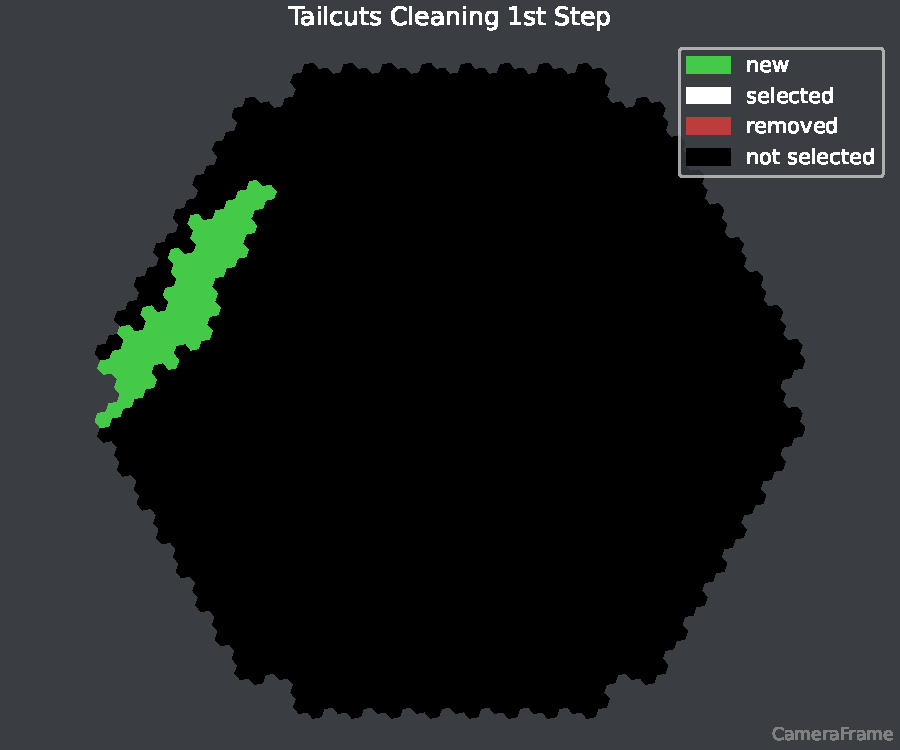
\includegraphics[width=\textwidth]{plots/cleaners/tail_1.pdf}
      }
      \only<5>{
        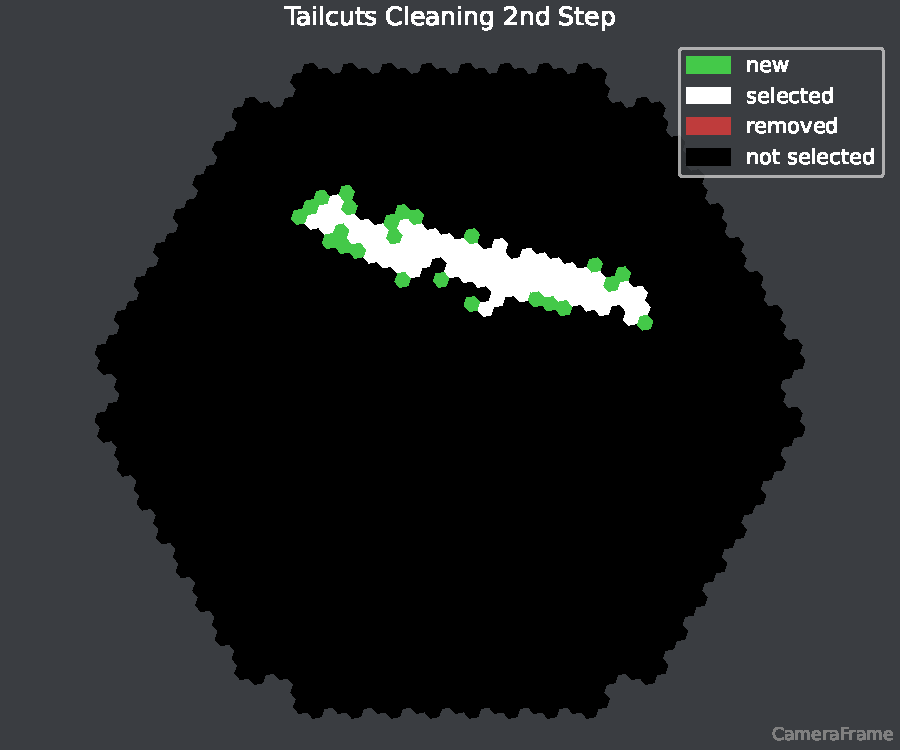
\includegraphics[width=\textwidth]{plots/cleaners/tail_2.pdf}
      }
      \only<6>{
      \begin{itemize}
        \setlength\itemsep{1em}
        \item \code{white!50!black}{TailcutsImageCleaner}
        \item \code{white}{MARSImageCleaner}
        \item \code{white!50!black}{FACTImageCleaner}
        \item \code{white!50!black}{TimeConstrainedImageCleaner}
      \end{itemize}
      }
      \only<7>{
        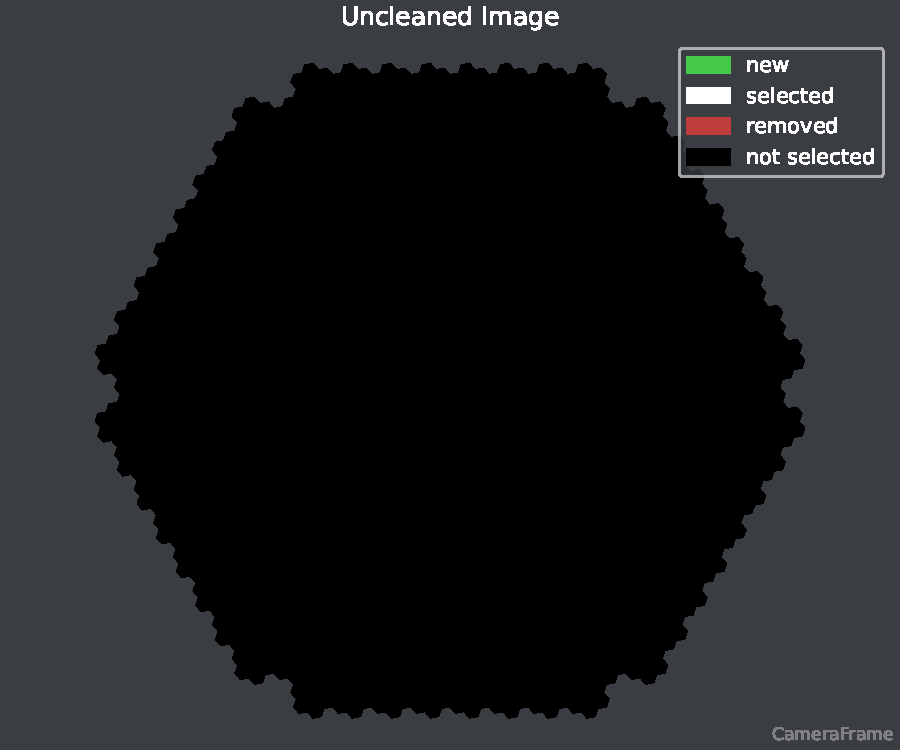
\includegraphics[width=\textwidth]{plots/cleaners/null_image.pdf}
      }
      \only<8>{
        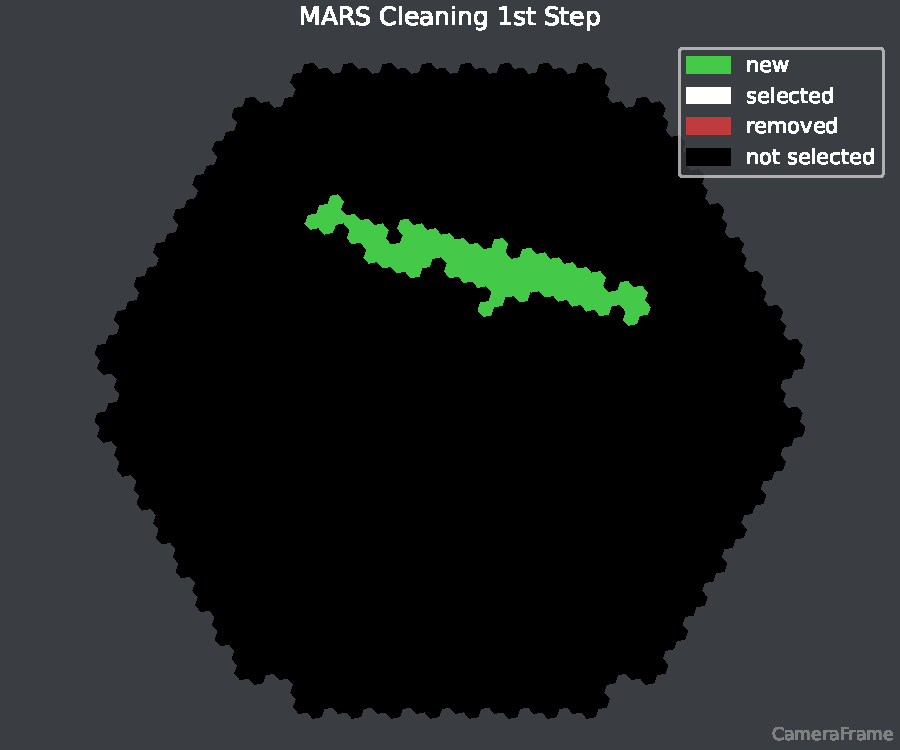
\includegraphics[width=\textwidth]{plots/cleaners/mars_1.pdf}
      }
      \only<9>{
        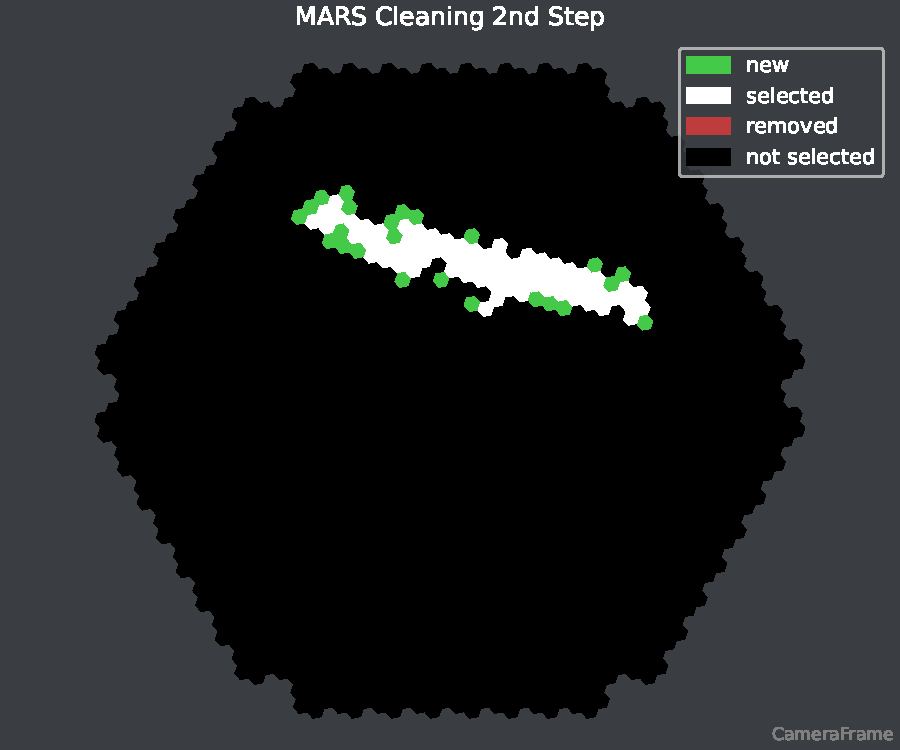
\includegraphics[width=\textwidth]{plots/cleaners/mars_2.pdf}
      }
      \only<10>{
        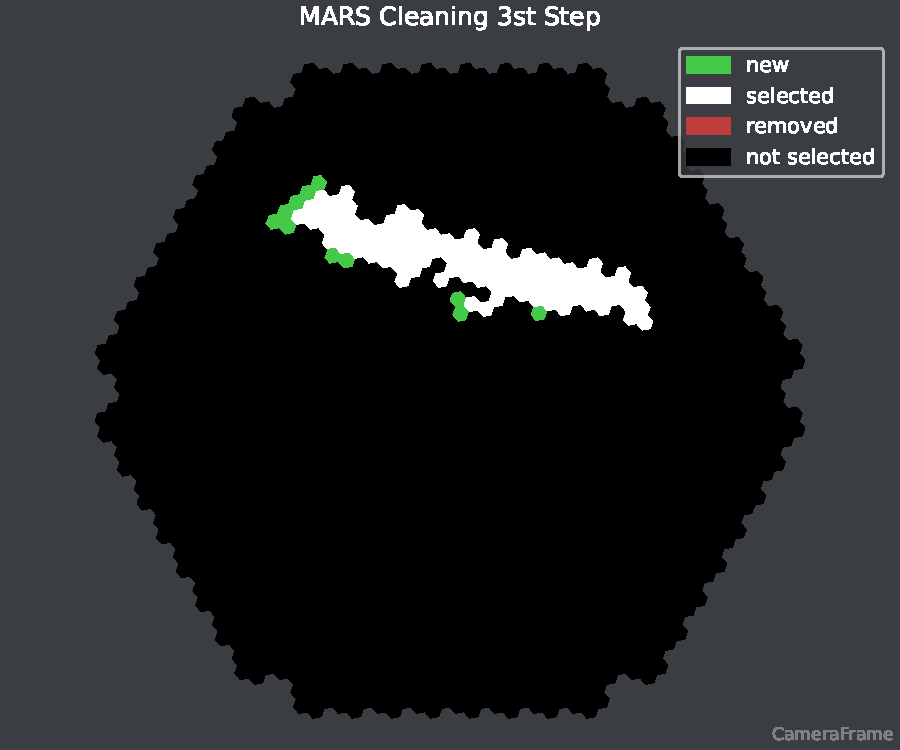
\includegraphics[width=\textwidth]{plots/cleaners/mars_3.pdf}
      }
      \only<11>{
      \begin{itemize}
        \setlength\itemsep{1em}
        \item \code{white!50!black}{TailcutsImageCleaner}
        \item \code{white!50!black}{MARSImageCleaner}
        \item \code{white}{FACTImageCleaner}
        \item \code{white!50!black}{TimeConstrainedImageCleaner}
      \end{itemize}
      }
      \only<12>{
        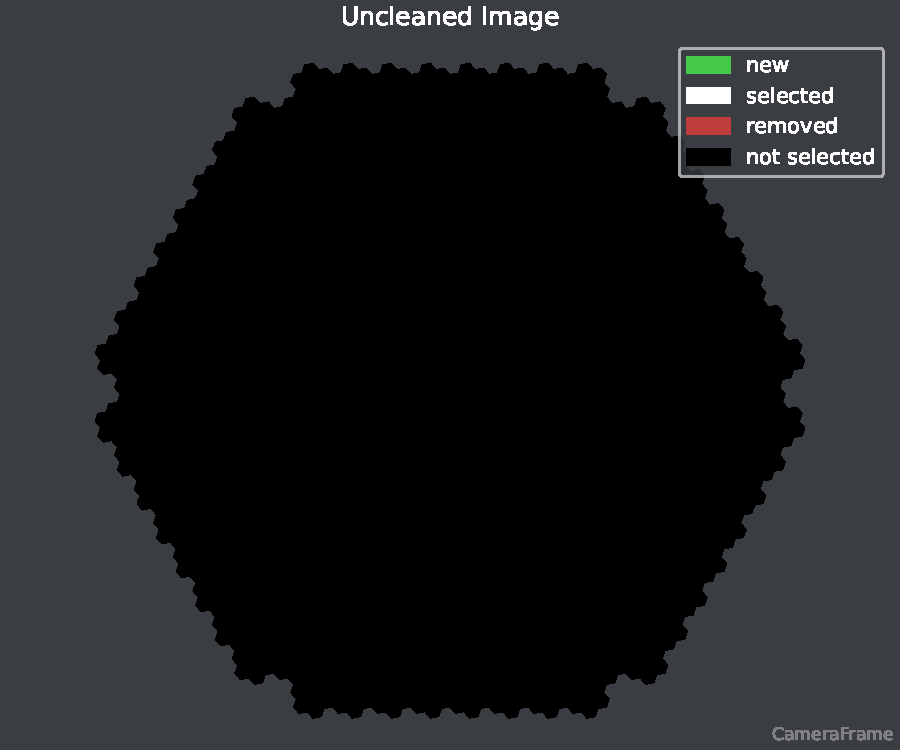
\includegraphics[width=\textwidth]{plots/cleaners/null_image.pdf}
      }
      \only<13>{
        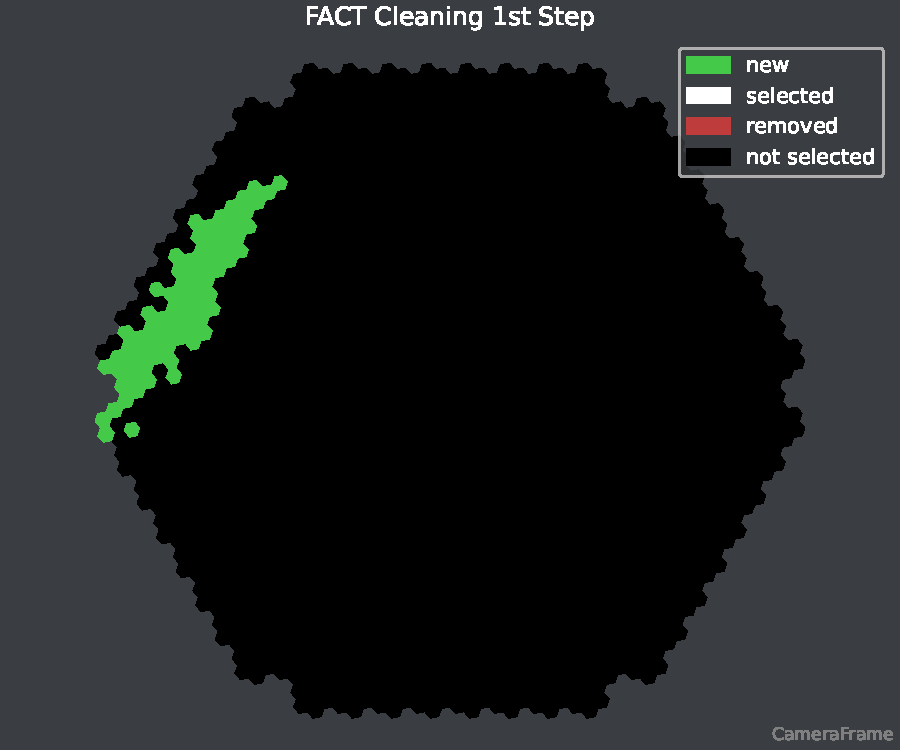
\includegraphics[width=\textwidth]{plots/cleaners/fact_1.pdf}
      }
      \only<14>{
        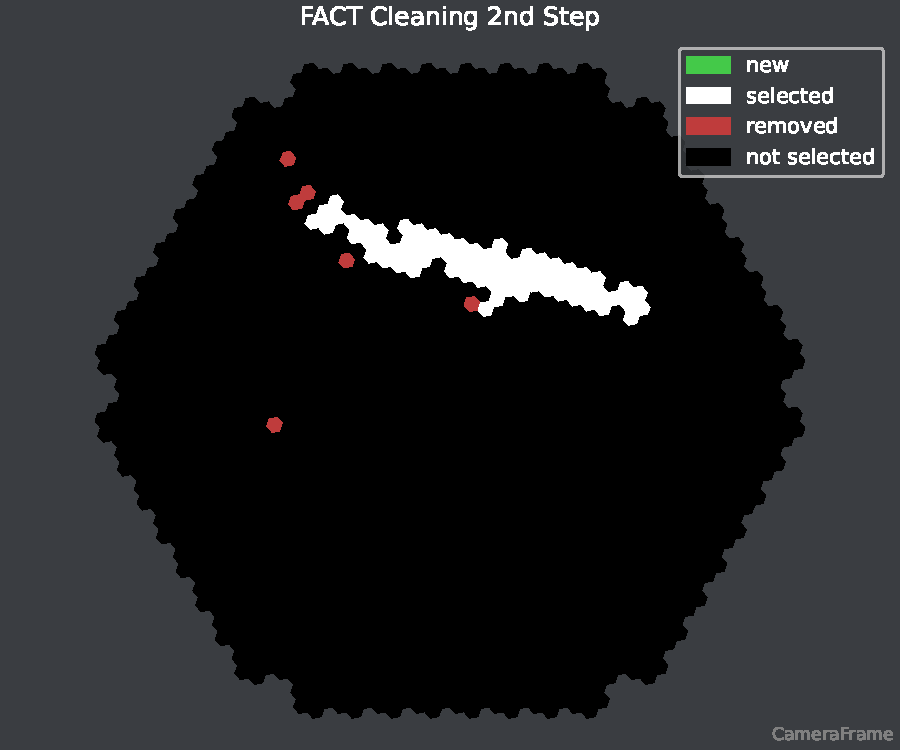
\includegraphics[width=\textwidth]{plots/cleaners/fact_2.pdf}
      }
      \only<15>{
        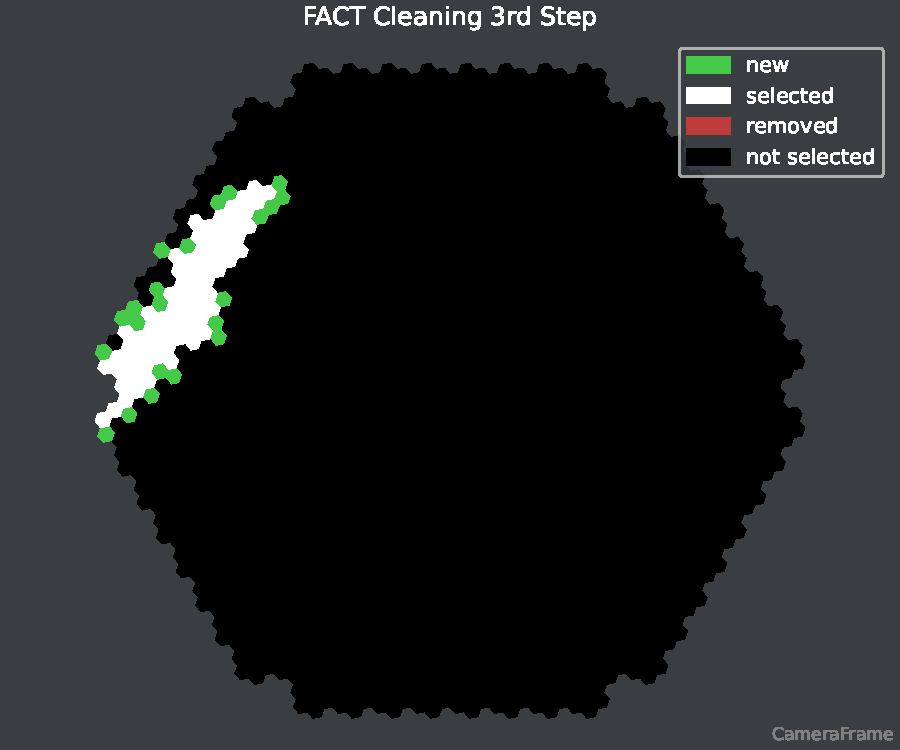
\includegraphics[width=\textwidth]{plots/cleaners/fact_3.pdf}
      }
      \only<16>{
        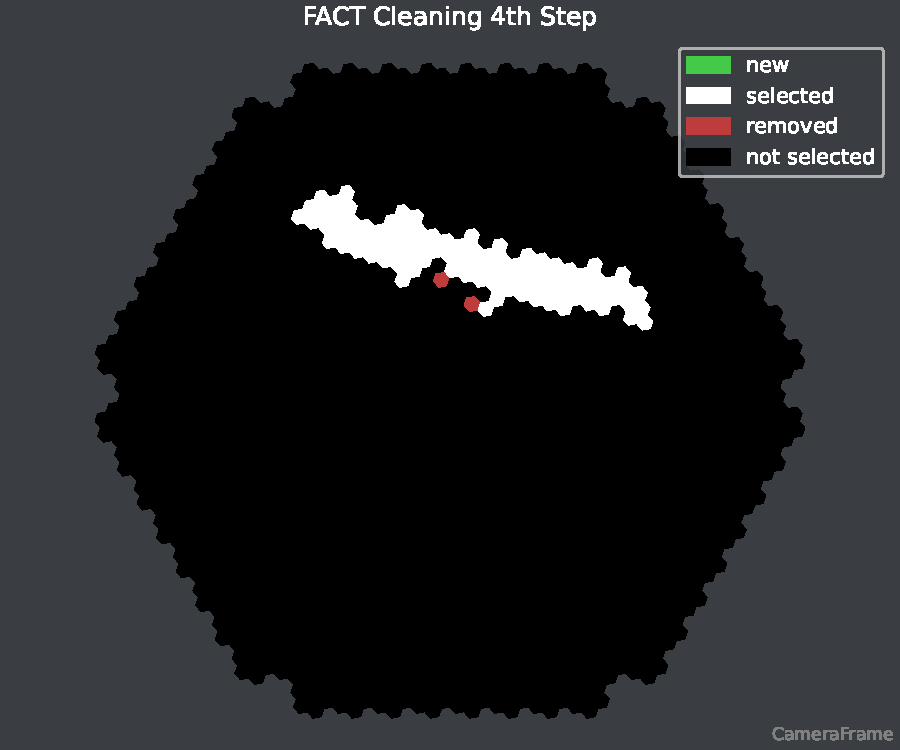
\includegraphics[width=\textwidth]{plots/cleaners/fact_4.pdf}
      }
      \only<17>{
        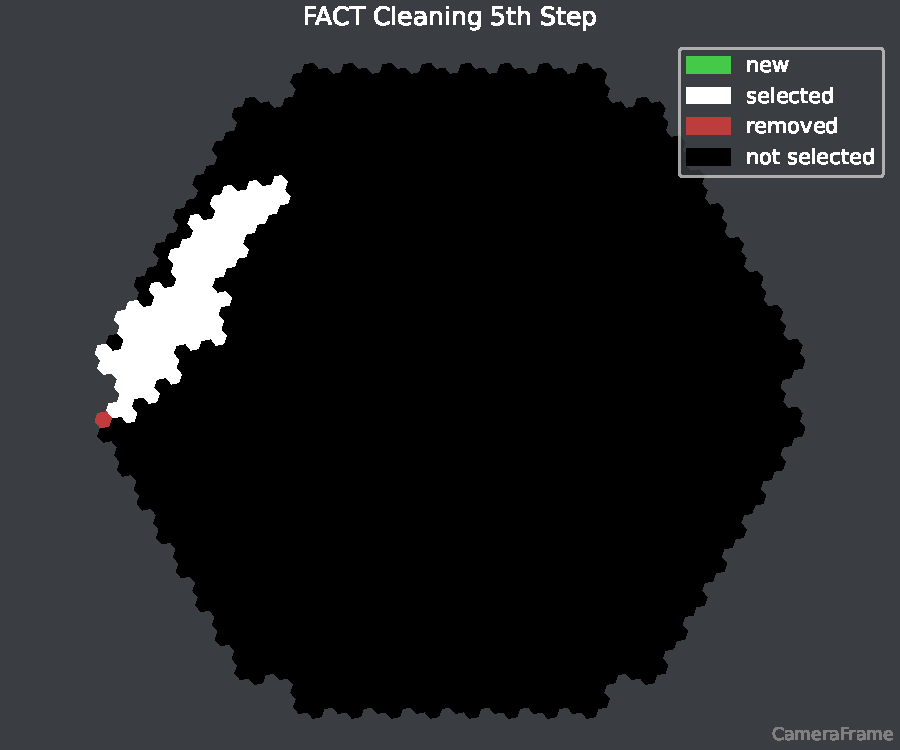
\includegraphics[width=\textwidth]{plots/cleaners/fact_5.pdf}
      }
      \only<18>{
        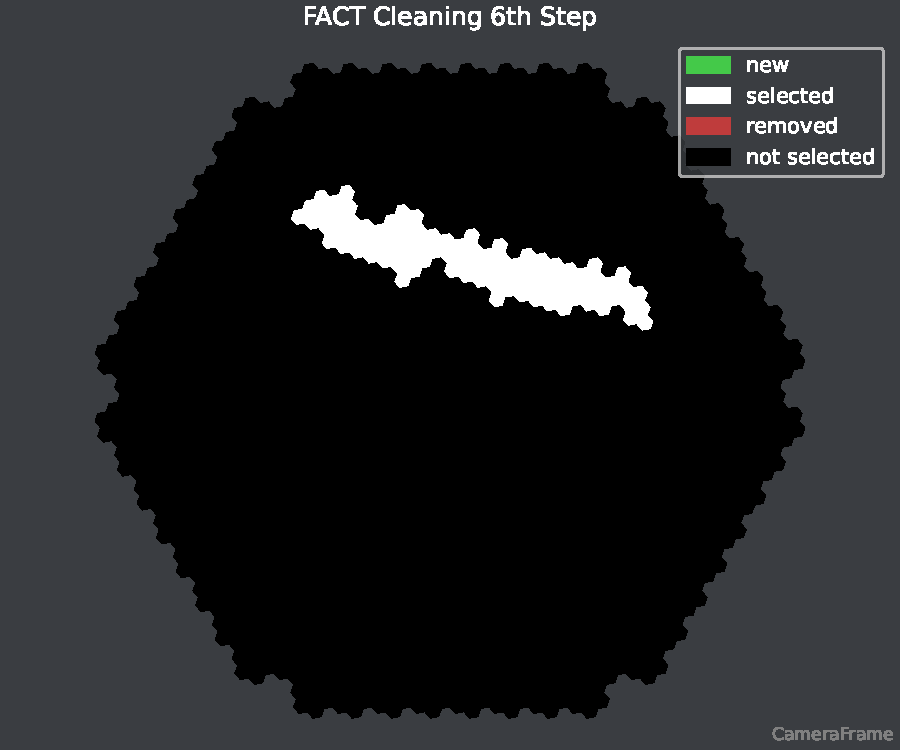
\includegraphics[width=\textwidth]{plots/cleaners/fact_6.pdf}
      }
      \only<19>{
      \begin{itemize}
        \setlength\itemsep{1em}
        \item \code{white!50!black}{TailcutsImageCleaner}
        \item \code{white!50!black}{MARSImageCleaner}
        \item \code{white!50!black}{FACTImageCleaner}
        \item \code{white}{TimeConstrainedImageCleaner}
      \end{itemize}
      }
      \only<20>{
        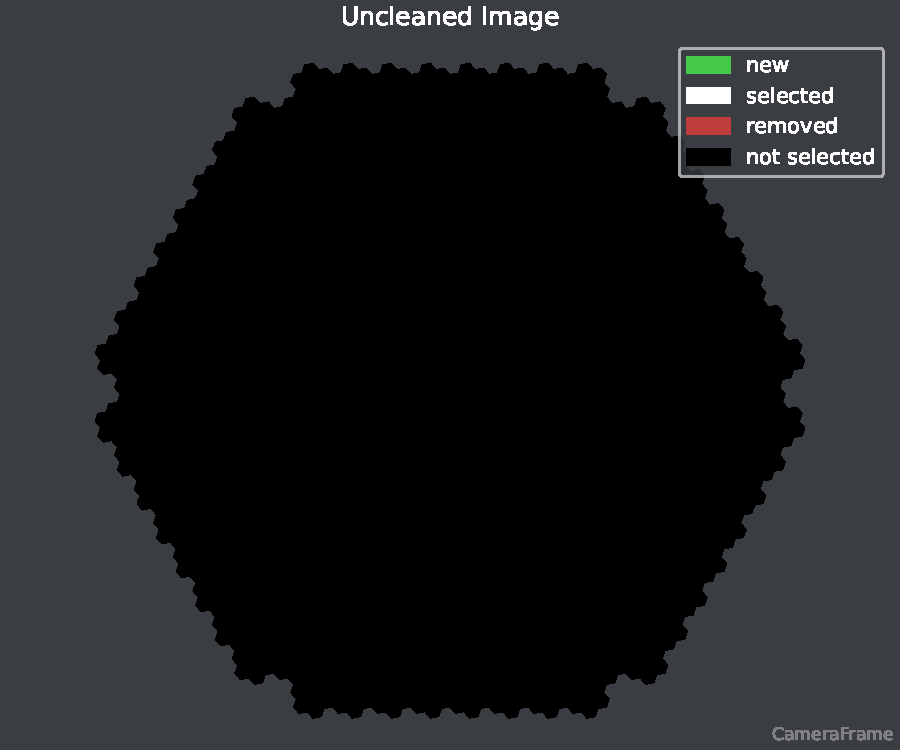
\includegraphics[width=\textwidth]{plots/cleaners/null_image.pdf}
      }
      \only<21>{
        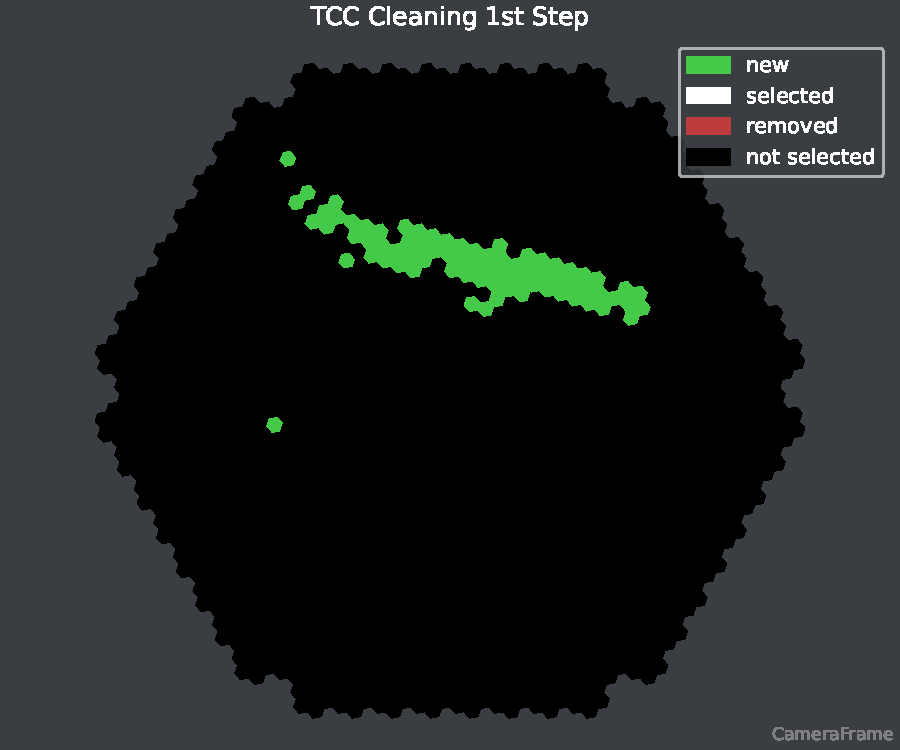
\includegraphics[width=\textwidth]{plots/cleaners/tcc_1.pdf}
      }
      \only<22>{
        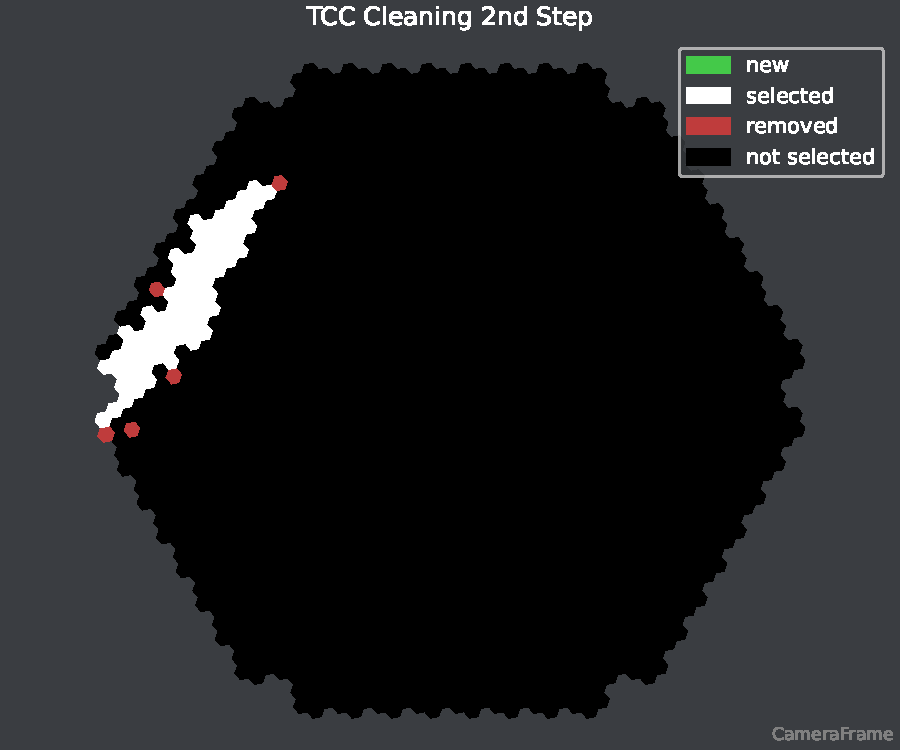
\includegraphics[width=\textwidth]{plots/cleaners/tcc_2.pdf}
      }
      \only<23>{
        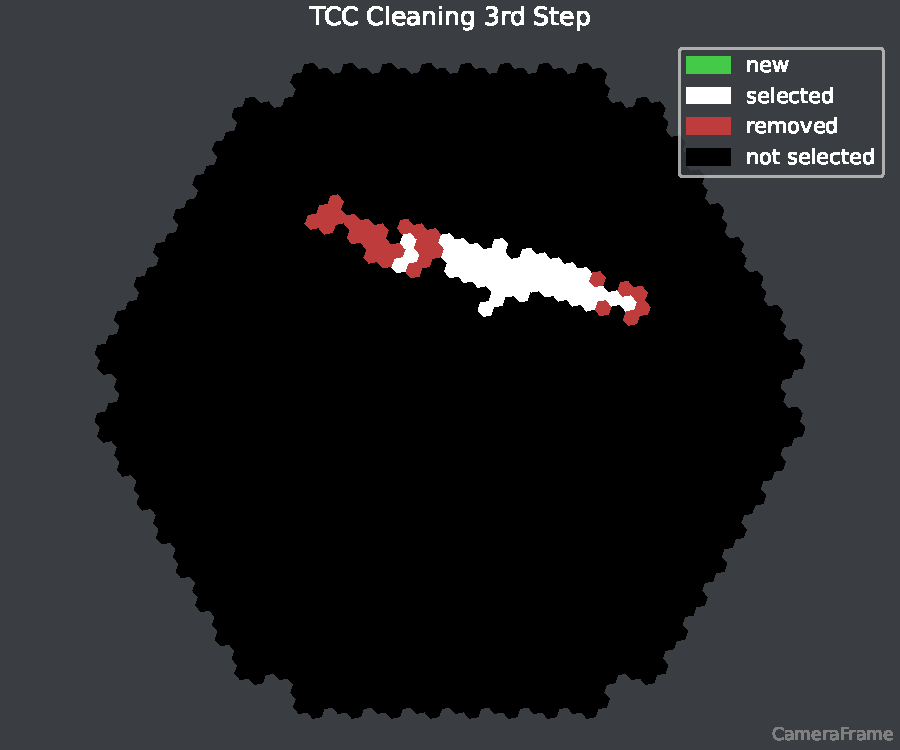
\includegraphics[width=\textwidth]{plots/cleaners/tcc_3.pdf}
      }
      \only<24>{
        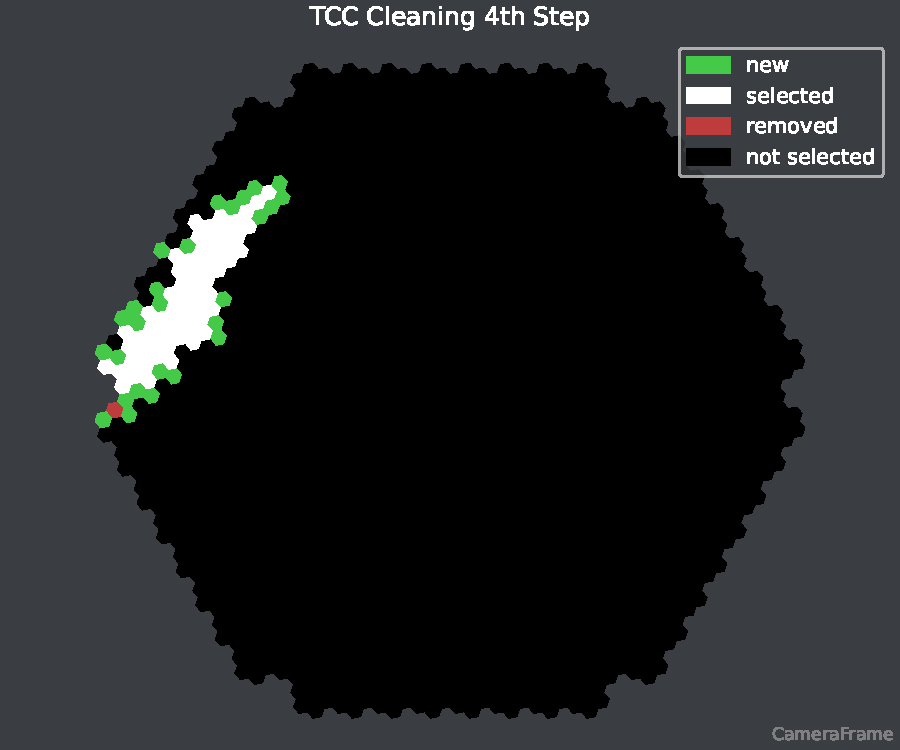
\includegraphics[width=\textwidth]{plots/cleaners/tcc_4.pdf}
      }
      \only<25>{
        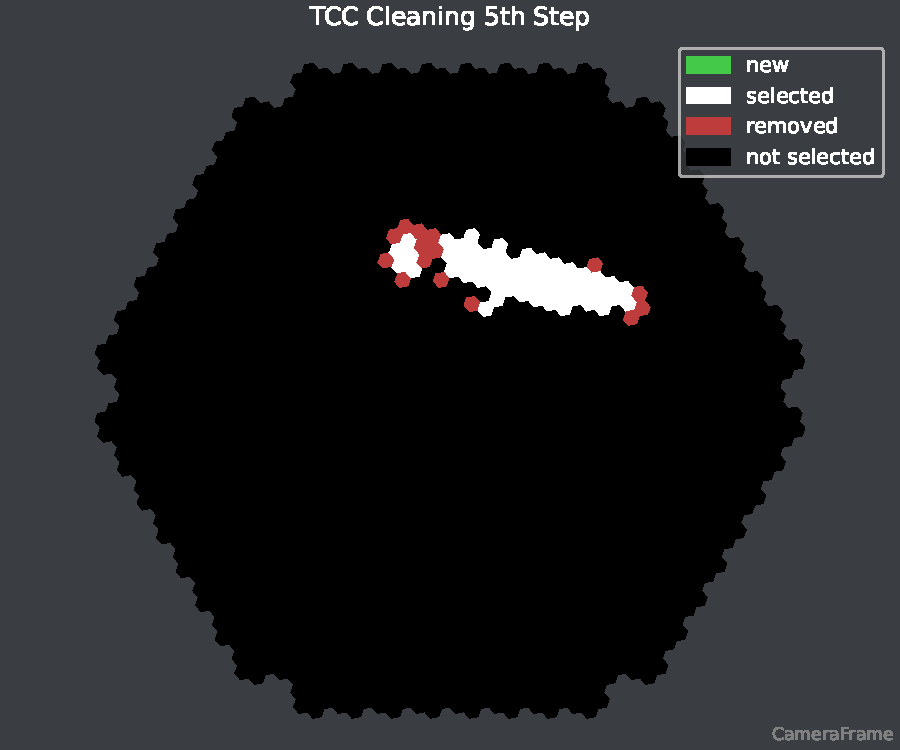
\includegraphics[width=\textwidth]{plots/cleaners/tcc_5.pdf}
      }
    \end{overlayarea}
    }
    \raisebox{10ex}{
    \begin{overlayarea}{0.58\textwidth}{3.5cm}
      \only<2>{
      \begin{enumerate}%TailcutsImageCleaner
        \item Selects pixels that pass the \code{white!70!black}{picture threshold}
        \item Adds pixels that pass the \code{white!70!black}{boundary threshold}
      \end{enumerate}
      }
      \only<3>{
      \begin{enumerate}%TailcutsImageCleaner
        \item \textcolor{white!50!black}{Selects pixels that pass the \code{white!35!black}{picture threshold}}
        \item \textcolor{white!50!black}{Adds pixels that pass the \code{white!35!black}{boundary threshold}}
      \end{enumerate}
      }
      \only<4>{
      \begin{enumerate}%TailcutsImageCleaner
        \item Selects pixels that pass the \code{white!70!black}{picture threshold}
        \item \textcolor{white!50!black}{Adds pixels that pass the \code{white!35!black}{boundary threshold}}
      \end{enumerate}
      }
      \only<5>{
      \begin{enumerate}%TailcutsImageCleaner
        \item \textcolor{white!50!black}{Selects pixels that pass the \code{white!35!black}{picture threshold}}
        \item Adds pixels that pass the \code{white!70!black}{boundary threshold}
      \end{enumerate}
      }

      \only<6>{
      \begin{enumerate}%MARSImageCleaner
        \item Selects pixels that pass a \code{white!70!black}{picture} and \code{white!70!black}{boundary threshold}, analogous to \code{white!70!black}{TailcutsImageCleaner}
        \item Adds pixels that are a neighbor of a neighbor of a core pixel, if they are above the \code{white!70!black}{boundary threshold}
      \end{enumerate}
      }
      \only<7>{
      \begin{enumerate}%MARSImageCleaner
        \item \textcolor{white!50!black}{Selects pixels that pass a \code{white!35!black}{picture} and \code{white!35!black}{boundary threshold}, analogous to \code{white!35!black}{TailcutsImageCleaner}}
        \item \textcolor{white!50!black}{Adds pixels that are a neighbor of a neighbor of a core pixel, if they are above the \code{white!35!black}{boundary threshold}}
      \end{enumerate}
      }
      \only<8-9>{
      \begin{enumerate}%MARSImageCleaner
        \item Selects pixels that pass a \code{white!70!black}{picture} and \code{white!70!black}{boundary threshold}, analogous to \code{white!70!black}{TailcutsImageCleaner}
        \item \textcolor{white!50!black}{Adds pixels that are a neighbor of a neighbor of a core pixel, if they are above the \code{white!35!black}{boundary threshold}}
      \end{enumerate}
      }
      \only<10>{
      \begin{enumerate}%MARSImageCleaner
        \item \textcolor{white!50!black}{Selects pixels that pass a \code{white!35!black}{picture} and \code{white!35!black}{boundary threshold}, analogous to \code{white!35!black}{TailcutsImageCleaner}}
        \item Adds pixels that are a neighbor of a neighbor of a core pixel, if they are above the \code{white!70!black}{boundary threshold}
      \end{enumerate}
      }
      \only<11>{
      \begin{enumerate}%FACTImageCleaner
        \item Finds all pixels that contain more photons than the \code{white!70!black}{picture threshold}
        \item Removes pixels with less than \(N\) neighbors
        \item Adds remaining neighbors that are above the \code{white!70!black}{boundary threshold}
        \item Removes pixels that have less than \(N\) neighbors, that arrive within a given timeframe (here: \SI{5}{\nano\second})
        \item Removes pixels that have less than \(N\) neighbors
        \item Removes pixels that have less than \(N\) neighbors, arriving within a given timeframe (same as in step 4)
      \end{enumerate}
      }
      \only<12>{
      \begin{enumerate}%FACTImageCleaner
        \item \textcolor{white!50!black}{Finds all pixels that contain more photons than the \code{white!35!black}{picture threshold}}
        \item \textcolor{white!50!black}{Removes pixels with less than \(N\) neighbors}
        \item \textcolor{white!50!black}{Adds remaining neighbors that are above the \code{white!35!black}{boundary threshold}}
        \item \textcolor{white!50!black}{Removes pixels that have less than \(N\) neighbors, that arrive within a given timeframe (here: \SI{5}{\nano\second})}
        \item \textcolor{white!50!black}{Removes pixels that have less than \(N\) neighbors}
        \item \textcolor{white!50!black}{Removes pixels that have less than \(N\) neighbors, arriving within a given timeframe (same as in step 4)}
      \end{enumerate}
      }
      \only<13>{
      \begin{enumerate}%FACTImageCleaner
        \item Finds all pixels that contain more photons than the \code{white!70!black}{picture threshold}
        \item \textcolor{white!50!black}{Removes pixels with less than \(N\) neighbors}
        \item \textcolor{white!50!black}{Adds remaining neighbors that are above the \code{white!35!black}{boundary threshold}}
        \item \textcolor{white!50!black}{Removes pixels that have less than \(N\) neighbors, that arrive within a given timeframe (here: \SI{5}{\nano\second})}
        \item \textcolor{white!50!black}{Removes pixels that have less than \(N\) neighbors}
        \item \textcolor{white!50!black}{Removes pixels that have less than \(N\) neighbors, arriving within a given timeframe (same as in step 4)}
      \end{enumerate}
      }
      \only<14>{
      \begin{enumerate}%FACTImageCleaner
        \item \textcolor{white!50!black}{Finds all pixels that contain more photons than the \code{white!35!black}{picture threshold}}
        \item Removes pixels with less than \(N\) neighbors
        \item \textcolor{white!50!black}{Adds remaining neighbors that are above the \code{white!35!black}{boundary threshold}}
        \item \textcolor{white!50!black}{Removes pixels that have less than \(N\) neighbors, that arrive within a given timeframe (here: \SI{5}{\nano\second})}
        \item \textcolor{white!50!black}{Removes pixels that have less than \(N\) neighbors}
        \item \textcolor{white!50!black}{Removes pixels that have less than \(N\) neighbors, arriving within a given timeframe (same as in step 4)}
      \end{enumerate}
      }
      \only<15>{
      \begin{enumerate}%FACTImageCleaner
        \item \textcolor{white!50!black}{Finds all pixels that contain more photons than the \code{white!35!black}{picture threshold}}
        \item \textcolor{white!50!black}{Removes pixels with less than \(N\) neighbors}
        \item Adds remaining neighbors that are above the \code{white!70!black}{boundary threshold}
        \item \textcolor{white!50!black}{Removes pixels that have less than \(N\) neighbors, that arrive within a given timeframe (here: \SI{5}{\nano\second})}
        \item \textcolor{white!50!black}{Removes pixels that have less than \(N\) neighbors}
        \item \textcolor{white!50!black}{Removes pixels that have less than \(N\) neighbors, arriving within a given timeframe (same as in step 4)}
      \end{enumerate}
      }
      \only<16>{
      \begin{enumerate}%FACTImageCleaner
        \item \textcolor{white!50!black}{Finds all pixels that contain more photons than the \code{white!35!black}{picture threshold}}
        \item \textcolor{white!50!black}{Removes pixels with less than \(N\) neighbors}
        \item \textcolor{white!50!black}{Adds remaining neighbors that are above the \code{white!35!black}{boundary threshold}}
        \item Removes pixels that have less than \(N\) neighbors, that arrive within a given timeframe (here: \SI{5}{\nano\second})
        \item \textcolor{white!50!black}{Removes pixels that have less than \(N\) neighbors}
        \item \textcolor{white!50!black}{Removes pixels that have less than \(N\) neighbors, arriving within a given timeframe (same as in step 4)}
      \end{enumerate}
      }
      \only<17>{
      \begin{enumerate}%FACTImageCleaner
        \item \textcolor{white!50!black}{Finds all pixels that contain more photons than the \code{white!35!black}{picture threshold}}
        \item \textcolor{white!50!black}{Removes pixels with less than \(N\) neighbors}
        \item \textcolor{white!50!black}{Adds remaining neighbors that are above the \code{white!35!black}{boundary threshold}}
        \item \textcolor{white!50!black}{Removes pixels that have less than \(N\) neighbors, that arrive within a given timeframe (here: \SI{5}{\nano\second})}
        \item Removes pixels that have less than \(N\) neighbors
        \item \textcolor{white!50!black}{Removes pixels that have less than \(N\) neighbors, arriving within a given timeframe (same as in step 4)}
      \end{enumerate}
      }
      \only<18>{
      \begin{enumerate}%FACTImageCleaner
        \item \textcolor{white!50!black}{Finds all pixels that contain more photons than the \code{white!35!black}{picture threshold}}
        \item \textcolor{white!50!black}{Removes pixels with less than \(N\) neighbors}
        \item \textcolor{white!50!black}{Adds remaining neighbors that are above the \code{white!35!black}{boundary threshold}}
        \item \textcolor{white!50!black}{Removes pixels that have less than \(N\) neighbors, that arrive within a given timeframe (here: \SI{5}{\nano\second})}
        \item \textcolor{white!50!black}{Removes pixels that have less than \(N\) neighbors}
        \item Removes pixels that have less than \(N\) neighbors, arriving within the given timeframe (same as in step 4)
      \end{enumerate}
      }
      \only<19>{
      \begin{enumerate}%TimeConstrainedImageCleaner
        \item Finds all core pixels above the \code{white!70!black}{picture threshold}
        \item Removes pixels with less than \(N\) neighbors
        \item Keeps all pixels that arrive within a time limit of the average arrival time (\code{white!70!black}{time_limit_core}: \SI{4.5}{\nano\second})
        \item Finds all neighbboring pixels above the \code{white!70!black}{boundary threshold}
        \item Removes all pixels with less than \(N\) neighbors arriving within a given timeframe (\code{white!70!black}{time_limit_boundary}: \SI{1.5}{\nano\second})
      \end{enumerate}
      }
      \only<20>{
      \begin{enumerate}%TimeConstrainedImageCleaner
        \item \textcolor{white!50!black}{Finds all core pixels above the \code{white!35!black}{picture threshold}}
        \item \textcolor{white!50!black}{Removes pixels with less than \(N\) neighbors}
        \item \textcolor{white!50!black}{Keeps all pixels that arrive within a time limit of the average arrival time (\code{white!35!black}{time_limit_core}: \SI{4.5}{\nano\second})}
        \item \textcolor{white!50!black}{Finds all neighbboring pixels above the \code{white!35!black}{boundary threshold}}
        \item \textcolor{white!50!black}{Removes all pixels with less than \(N\) neighbors arriving within a given timeframe (\code{white!35!black}{time_limit_boundary}: \SI{1.5}{\nano\second})}
      \end{enumerate}
      }
      \only<21>{
      \begin{enumerate}%TimeConstrainedImageCleaner
        \item Finds all core pixels above the \code{white!70!black}{picture threshold}
        \item \textcolor{white!50!black}{Removes pixels with less than \(N\) neighbors}
        \item \textcolor{white!50!black}{Keeps all pixels that arrive within a time limit of the average arrival time (\code{white!35!black}{time_limit_core}: \SI{4.5}{\nano\second})}
        \item \textcolor{white!50!black}{Finds all neighbboring pixels above the \code{white!35!black}{boundary threshold}}
        \item \textcolor{white!50!black}{Removes all pixels with less than \(N\) neighbors arriving within a given timeframe (\code{white!35!black}{time_limit_boundary}: \SI{1.5}{\nano\second})}
      \end{enumerate}
      }
      \only<22>{
      \begin{enumerate}%TimeConstrainedImageCleaner
        \item \textcolor{white!50!black}{Finds all core pixels above the \code{white!35!black}{picture threshold}}
        \item Removes pixels with less than \(N\) neighbors
        \item \textcolor{white!50!black}{Keeps all pixels that arrive within a time limit of the average arrival time (\code{white!35!black}{time_limit_core}: \SI{4.5}{\nano\second})}
        \item \textcolor{white!50!black}{Finds all neighbboring pixels above the \code{white!35!black}{boundary threshold}}
        \item \textcolor{white!50!black}{Removes all pixels with less than \(N\) neighbors arriving within a given timeframe (\code{white!35!black}{time_limit_boundary}: \SI{1.5}{\nano\second})}
      \end{enumerate}
      }
      \only<23>{
      \begin{enumerate}%TimeConstrainedImageCleaner
        \item \textcolor{white!50!black}{Finds all core pixels above the \code{white!35!black}{picture threshold}}
        \item \textcolor{white!50!black}{Removes pixels with less than \(N\) neighbors}
        \item Keeps all pixels that arrive within a time limit of the average arrival time (\code{white!70!black}{time_limit_core}: \SI{4.5}{\nano\second})
        \item \textcolor{white!50!black}{Finds all neighbboring pixels above the \code{white!35!black}{boundary threshold}}
        \item \textcolor{white!50!black}{Removes all pixels with less than \(N\) neighbors arriving within a given timeframe (\code{white!35!black}{time_limit_boundary}: \SI{1.5}{\nano\second})}
      \end{enumerate}
      }
      \only<24>{
      \begin{enumerate}%TimeConstrainedImageCleaner
        \item \textcolor{white!50!black}{Finds all core pixels above the \code{white!35!black}{picture threshold}}
        \item \textcolor{white!50!black}{Removes pixels with less than \(N\) neighbors}
        \item \textcolor{white!50!black}{Keeps all pixels that arrive within a time limit of the average arrival time (\code{white!35!black}{time_limit_core}: \SI{4.5}{\nano\second})}
        \item Finds all neighbboring pixels above the \code{white!70!black}{boundary threshold}
        \item \textcolor{white!50!black}{Removes all pixels with less than \(N\) neighbors arriving within a given timeframe (\code{white!35!black}{time_limit_boundary}: \SI{1.5}{\nano\second})}
      \end{enumerate}
      }
      \only<25>{
      \begin{enumerate}%TimeConstrainedImageCleaner
        \item \textcolor{white!50!black}{Finds all core pixels above the \code{white!35!black}{picture threshold}}
        \item \textcolor{white!50!black}{Removes pixels with less than \(N\) neighbors}
        \item \textcolor{white!50!black}{Keeps all pixels that arrive within a time limit of the average arrival time (\code{white!35!black}{time_limit_core}: \SI{4.5}{\nano\second})}
        \item \textcolor{white!50!black}{Finds all neighbboring pixels above the \code{white!35!black}{boundary threshold}}
        \item Removes all pixels with less than \(N\) neighbors arriving within a given timeframe (\code{white!70!black}{time_limit_boundary}: \SI{1.5}{\nano\second})
      \end{enumerate}
      }
    \end{overlayarea}
    }
  \end{frame}